
Our work, \Tool{}, advances grammar-guided LLM generation techniques by introducing a framework that utilizes grammar symbols as abstractions for iterating the generation both forward and backward. 
Unlike current grammar-guided tools, which struggle to detect semantic violations and cannot pause generation at intermediate points, our approach enables users to navigate output based on grammatical structures. 
This flexibility allows for more effective handling of semantically incorrect outputs without the need to restart generation from scratch.
% outline
In this section, we first outline the \Tool{} interface that supports this navigation. 
Following that, we discuss the technical challenges and the algorithm that efficiently facilitates these functionalities.

\begin{figure}[!t]
\centering
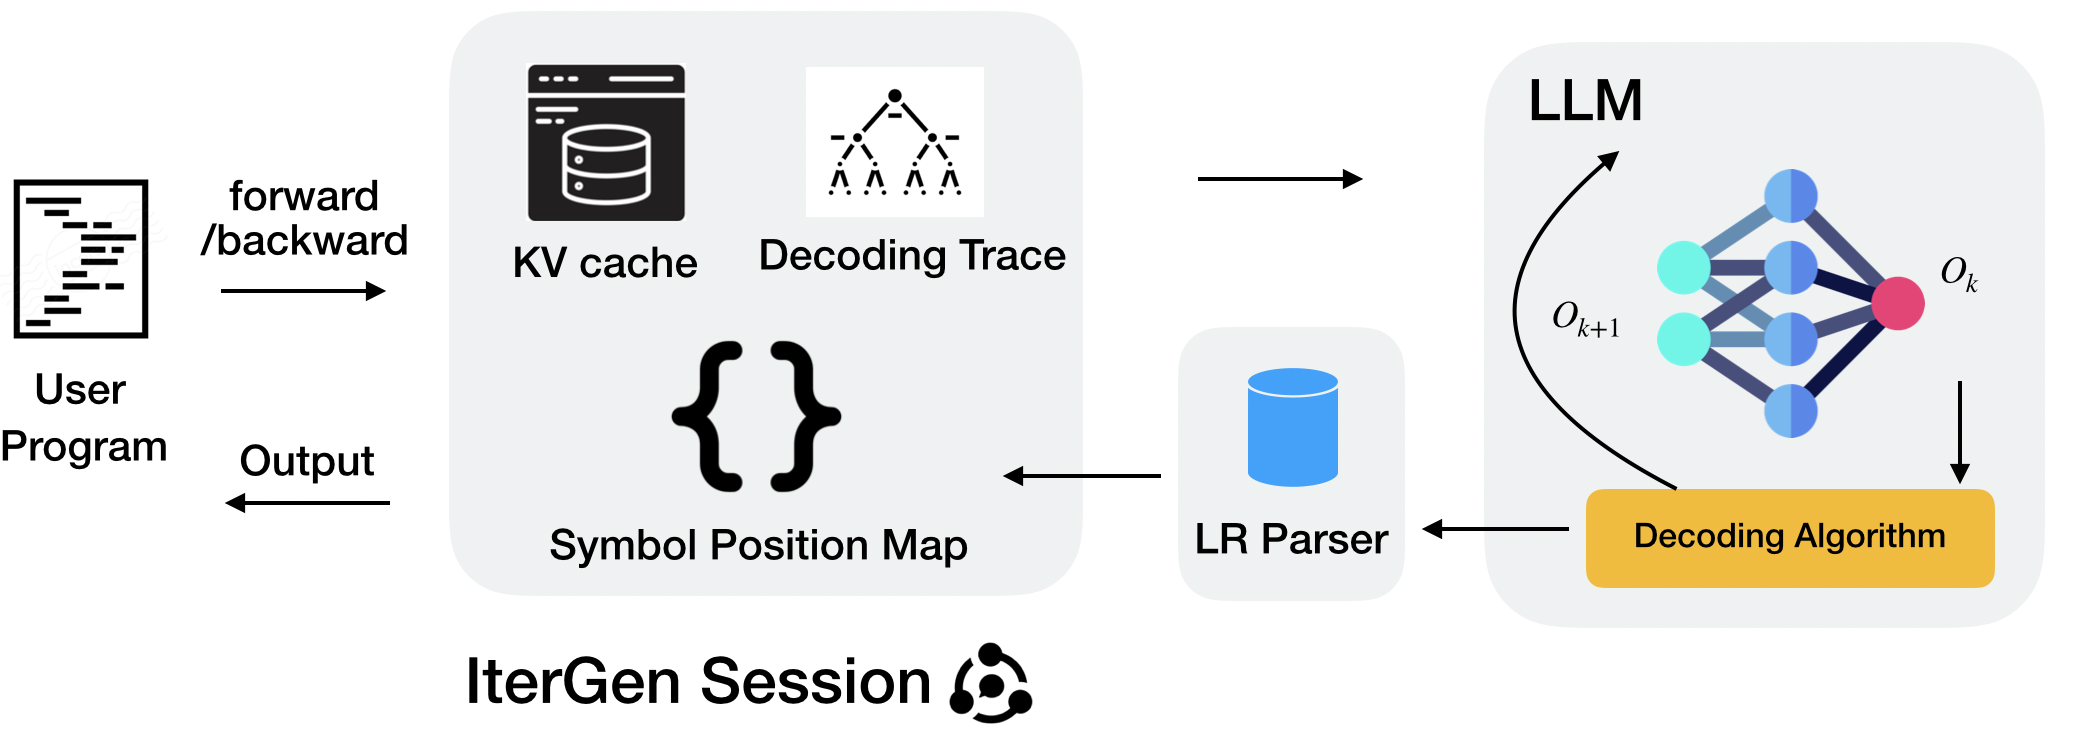
\includegraphics[width=13cm]{images/workflow.png}
\vspace{-.1in}
\caption{
In our workflow, a user program utilizing the \Tool{} manages LLM generation through forward and backward calls. 
For each prompt $O_0$, \Tool{} maintains a session that includes a decoding trace, a symbol position map, and a key-value (KV) cache.
Using the LR parser \Tool{} incrementally parses partially generated output $O_k$ and continuously updates the symbol position map to track the locations of symbols from the grammar in $O_k$. 
} 
\label{fig:workflow}
\vspace{-.1in}
\end{figure}


\subsection{\Tool{} Interface}

% \sasa{Call it interface? Library functions sounds like we're doing a tool paper...}
% Talk about forward, backward, and view 
% An \Tool{} session is initialized by providing a prompt and a grammar. 
Given a prompt and the grammar, a program using \Tool{}  can specify various generation parameters such as the decoding algorithm, temperature, and other supported options. 
\Tool{} simplifies generation with three key functions: \mbox{\str{forward}, \str{backward}, and \str{view}.}

The \str{forward} function accepts a stop symbol from the grammar, which can be either terminal or non-terminal, along with a count. 
The LLM will generate until the number of new specified stop symbols in the generation reaches the specified count. 
The generation process may stop earlier if the model produces an EOS token or meets other stopping conditions, such as a maximum token limit.
Additionally, the generation parameters such as the decoding algorithm and temperature can be adjusted for each \str{forward} call.
Consequently, a \Tool{} program can sample each line in a program or a sentence in natural language text with a different decoding method.

The \str{backward} function also takes a grammar symbol and count as arguments. 
It allows the program to backtrack the generation process by the given number of specified symbols, effectively removing part of the output.
The \str{view} function can be used to inspect all parts of the partial generation so far that correspond to a given grammar symbol. 
This is useful for checking whether the output meets certain criteria. 
If the desired properties are not met, the user can invoke \str{backward} to backtrack the generation accordingly.

% Give an example of how rejection sampling can be used here
\noindent\textbf{Example Grammar:}

\begin{wrapfigure}{l}{0.6\textwidth}
\vspace{-.1in}
\begin{minipage}{0.6\textwidth}
    \begin{tcblisting}{
        listing only, 
        halign=left,
        listing engine=listings,
        title=\textbf{\small English text EBNF grammar},
        colbacktitle=blue!30!white, 
        coltitle=black,
        left=0pt,               % Left inner padding
        right=0mm,              % Right inner padding
        top=0mm,                % Reduce top margin
        bottom=0mm,             % Reduce bottom margin
        boxsep=1mm,
        width=\textwidth,
        listing options={style=EBNF},
        label={fig:overview_grammar},
    }
    **paragraph**: sentence+
    **sentence**: word+ sentence_end
    **word**: /[a-zA-Z0-9]+/ | other_punctuations
    **sentence_end**: "." | "!" | "?"
    **other_punctuations**: "," | ";" | ":" | "'" | "\""
    % ignore " "
    \end{tcblisting}
    \label{fig:ebnf_grammar}
\end{minipage}
\vspace{-.25in}
\end{wrapfigure}

Consider an example of grammar using the Lark EBNF syntax.
The grammar defines a simple English text paragraph. 
It consists of production rules where a \str{paragraph} is defined as one or more \str{sentences}. 
Each \str{sentence} is constructed from one or more \str{words} followed by a \str{sentence\_end} punctuation mark. 
% The \str{word} can be composed of alphanumeric characters and include specific punctuation symbols. 
In this grammar, symbols such as \str{paragraph} and \str{sentence} are non-terminals, meaning they can expand into other symbols according to the defined production rules. 
Conversely, symbols such as \str{.}, \str{!}, and \str{?} are terminals, as they cannot be further expanded. 

For the given example, a \str{forward(stop\_symbol="sentence")} would ensure that LLM generation stops after generating a sentence (default value of count is 1). 
A \str{backward("word", num=2)} function call would ensure that the generation moves backward by a unit of 2 words. 
A \str{view("word")} call would return a list of all words in the current generation.
These three functions can be effectively combined to create more complex LLM generation algorithms. 
For instance, one could implement a rejection sampling algorithm that backtracks until a specified criterion is met for a particular component of the output. 


\subsection{\Tool{} Algorithm}

Given a grammar $G$, let $\mathcal{S}$ denote the set of symbols corresponding to the terminals and non-terminals of the grammar.
Further, let $C: \alphabets^* \times \mathcal{S} \to \mathbb{I}$ be a function that represents the count of grammar symbol $S$ on parsing a string. 
i.e. if $C(O_i, S) = n$, then there are $n$ occurrences of $S$ in the partial parsing of $O_i$ with grammar $G$.
We use this to define the \Tool{} functions formally.

\textbf{Forward function:}
Let $ O_i \in \alphabets^* $ be the output string before the forward operation, and let $O_b \in \alphabets^*$ be the output after the call to the backward function.
Let $ S \in \mathcal{S} $ be the target stop symbol and $ n \in \mathbb{I}$ be an integer.
Given $ O_f = \text{\str{forward}}(S, n) $, the output $ O_f $ is formed by appending a suffix $ \Delta \in \alphabets^* $ to $ O_i $, such that $ O_f = O_i + \Delta $. Formally,

\begin{enumerate}
    \item $ C(O_f, S) - C(O_i, S) = n $, there are exactly $ n $ additional occurrences of the symbol $ S \in \mathcal{S} $; or 
    \item The generation stops at $ O_f $ when a termination condition is met, typically when the model generates an EOS token or reaches a maximum length. In this case, $ C(O_f, S) - C(O_i, S) < n $.
\end{enumerate}

\textbf{Backward function:} Similarly, let $ O_i \in \alphabets^* $ be the output string before the backward operation, and let $ O_b \in \alphabets^* $ be the output after the call to the backward function. 
Let $ S \in \mathcal{S} $ be the target stop symbol, and $ n \in \mathbb{I} $ be the input to the backward function. 
Given $ O_b = \text{\str{backward}}(S, n) $, the output $ O_b $ is the maximal prefix of $ O_i $ such that $ O_i = O_b + \Delta $, where $ C(\Delta, S) = n $. 
If $ C(O_i, S) < n $, indicating that $ O_i $ does not contain enough occurrences of $ S $, then the operation backtracks to the initial prompt $ O_0 $.


The detailed pseudocode for the forward and backward algorithm are presented in Appendix~\ref{sec:algos}. 

\noindent\textbf{Symbol Position Map:}
% \Tool{} utilizes a symbol position map to track the positions of grammar symbols throughout the generation process. 
% The primary challenge in navigating LLM generation using grammar symbols is token misalignment, where the terminals defined in the grammar do not align with the boundaries of the generated text. 
% % This misalignment complicates confirming the completion of a specific grammar symbol, as it often relies on the generation of subsequent tokens. 
% % For instance, if the partial LLM output is "we are human" the term "human" might extend into "humankind". 
% % In such cases, until the next token, such as " being" which starts with a whitespace is generated we cannot ascertain the word's completion.
% To address this misalignment, we employ a symbol position map that maps segments of the partial generation with their respective character positions. 
To enable the counting of the occurrence of grammar symbols in the LLM generation output we maintain the symbol position map that gets updated based on the LR parser reduce operations.
Formally, symbol position map is a mapping $\mathcal{D}: \mathcal{S'} \to \mathbb{I} \times \mathbb{I}$, where $\mathcal{S'}$ represents each occurrence of the grammar symbol in the current LLM-generated output, and $\mathbb{I} \times \mathbb{I}$ represents set of integer pairs. 
As the LLM generates tokens, the partially generated output is passed to an incremental LR parser. 
This parser first lexes the input, converting it into a list of lexical tokens (terminals). 
Since the parser works incrementally, at each LLM decoding step, newly generated lexical tokens are processed by the shift-reduce LR parser. 
\begin{wrapfigure}{r}{.43\textwidth}
    % \centering
    \vspace{-.1in}
    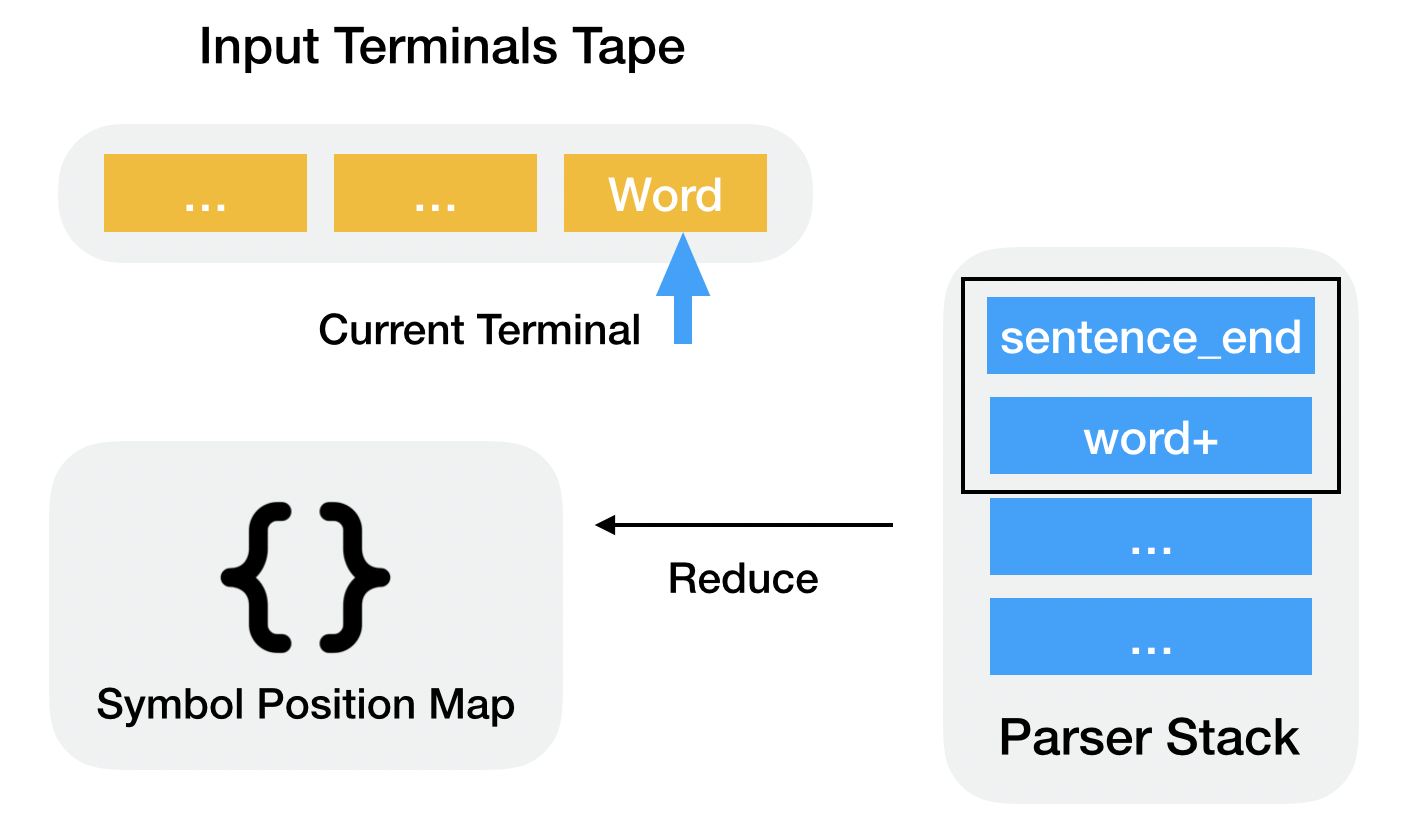
\includegraphics[width=0.43\textwidth]{images/parser.png}
    \caption{On every reduce operation the \Tool{} updates the position of the reduced symbol in the symbol position map.}
    \label{fig:parser}
     \vspace{-0.1in}
\end{wrapfigure}
Figure~\ref{fig:parser} illustrates these terminals on an input terminal tape.
The parser operates using a set of states and a parsing table that determines the next action—either shift or reduce—based on the symbols on the input tape. 
A shift operation updates the parser state and pushes the new terminal onto the stack. 
In contrast, a reduce operation corresponds to applying a grammar production rule, where elements at the top of the stack are reduced to a non-terminal. 
For example, if a production rule is $S \to S_1 S_2 \dots S_n$, where $S$ and each $ S_i$ are symbols in the grammar, a reduce operation replaces $S_1 S_2 \dots S_n$ on top of the stack with~$S$.

In \Tool{}, during a reduce operation, we update the symbol position map by recording the start and end positions of the reduced symbol. 
The start position of $S$ is taken from $S_1$, and the end position is taken from $S_n$.
Formally, the position of $S$ is calculated as: $\mathcal{D}(S) = (\mathcal{D}(S_1)_l, \mathcal{D}(S_n)_r)$.
Here, $\mathcal{D}(S_1)_l$ is the start position of $S_1$, and $\mathcal{D}(S_n)_r$ is the end position of $S_n$.
The LR parser then pushes $S$ onto the stack. 
As a result, every symbol added to the stack has an entry in the symbol position map. 
For any future reduce operations where these symbols are involved, their positions are recursively used to update the position of the newly reduced symbol.
In our example, when the top of the parser stack contains the symbols \str{word+} and \str{sentence\_end}, the production rule \str{sentence} $\to$ \str{word+} \str{sentence\_end} is applied to reduce the stack to \str{sentence}. 
At this point, we mark the positions of \mbox{the newly created \str{sentence} symbol.}

% detail 1
A subtle but important detail is that the reduce operation only occurs when the input tape contains the next terminal. 
In other words, a \str{sentence} is only reduced when the first word of the next sentence is already on the input tape (i.e., when the pointer reaches the end). This means that during token generation if we want \Tool{} to stop precisely at the end of a certain grammar symbol, LLM often needs to generate one extra token before halting. 
This extra token is then removed from the final output, and the \Tool{} session is updated accordingly.
Importantly, users of \Tool{} do not need to handle these internal mechanics—the generation will appear to stop exactly at the desired grammar symbol, ensuring accurate results without exposing the underlying complexity.

% \noindent\textbf{Token Misalignment:}


% Say how a shift-reduce parser pushes a symbol from the stack using certain lookahead

\noindent\textbf{Decoding Trace:}
% Recurrence penalty
We maintain a history of each session as a \emph{tree} of tokens, incorporating token indexes and associated metadata such as token probabilities. 
The trace includes a pointer to the last token.
During a forward call, a newly generated token is added as a child to the last token in the tree, effectively extending the session history. 
Conversely, during a backward call, the last token pointer is moved to a previous token position.
This trace storage is crucial when users navigate back and forth through LLM generation while performing rejection sampling, where achieving convergence to a different desired output may take longer. 
\add{
To expedite this process, we introduce a small recurrence penalty, denoted by $\gamma$, which is applied to the probabilities of previously selected tokens. 
Specifically, the probabilities are changed by multiplying them by $(1-\gamma)^\alpha$, where $\alpha$ is the number of times the token has been backtracked.
By utilizing a hyperparameter $\gamma$, we ensure that the model explores distinct paths each time it backtracks.
}

Additionally, LLMs use a Key-Value cache to store previously computed Key and Value matrices from the attention mechanism, enabling faster generation by reusing them for each new token.
% LLMs typically use a Key-Value cache mechanism to enhance generation speed. 
% KV-cache stores previously computed Key and Value vectors from attention calculations, allowing for their reuse in current token generation. 
During every \Tool{} session, we maintain the KV cache corresponding to the current generation and maintain it coherently with forward and backward calls. 
This enables efficient generation without having to go through the expensive \mbox{KV-cache prefill step again.}
% When a \str{backward} call is made, the cache is sliced to retain the cache corresponding to only the tokens that remain after the backward step, ensuring efficient future generations.

